\documentclass{beamer}

\usetheme{Warsaw}
%\usetheme{CambridgeUS}

% modification history
% created on 18 sep 2011
% modified on 25 mar

%\usepackage{amsfonts, amsmath, amssymb}

%\setbeamertemplate{theorems}[numbered]
%\setbeamertemplate{theorems}[ams style] 
\usepackage[skins,breakable]{tcolorbox}
%\usepackage[normalem]{ulem}

%\usefonttheme[onlymath]{serif}                     // change the style of math font 

%=============set slide number=================
\addtobeamertemplate{navigation symbols}{}{
    \usebeamerfont{footline}
    \usebeamercolor[fg]{footline}
    \hspace{1em}
    \insertframenumber/\inserttotalframenumber
}
\setbeamercolor{footline}{fg=black}
\setbeamerfont{footline}{series=\bfseries}


%=============set footline=====================
\setbeamertemplate{footline}
{
  \leavevmode%
  \hbox{%
  \begin{beamercolorbox}[wd=.55\paperwidth,ht=2.25ex,dp=1ex,center]{author in head/foot}%
    \usebeamerfont{author in head/foot}\insertshortauthor
  \end{beamercolorbox}%
  \begin{beamercolorbox}[wd=.45\paperwidth,ht=2.25ex,dp=1ex,center]{title in head/foot}%
    \usebeamerfont{title in head/foot}\insertshorttitle
  \end{beamercolorbox}}%
  \vskip0pt%
}

%creating a rectangle box def
\newtcbox{\mybox}[1][red]{arc=0pt,outer arc=0pt,colback=#1!10!white,colframe=#1!50!black, boxsep=0pt,left=1pt,right=1pt,top=2pt,bottom=2pt,boxrule=0pt,bottomrule=1pt,toprule=1pt}

\newtcbox{\xmybox}[1][red]{arc=7pt,colback=#1!10!white,colframe=#1!50!black,before upper={\rule[-3pt]{0pt}{10pt}},boxrule=1pt,boxsep=0pt,left=6pt,right=6pt,top=2pt,bottom=2pt}
%the ``on line'' option doesn't work. so omitting it

%===== spacing =====

\def\extraspacing{\vspace{2mm} \noindent}
\def\vgap{\vspace{2mm}}
\def\hgap{\textrm{\hspace{1mm}}}

%===== tabbing =====

\def\tab{\hspace{2mm}}
\def\tabpos{\hspace{4mm} \= \hspace{4mm} \= \hspace{4mm} \= \hspace{4mm} \=
\hspace{4mm} \= \hspace{4mm} \= \hspace{4mm} \= \hspace{4mm} \= \hspace{4mm}
\kill}
\newcommand{\mytab}[1]{\begin{tabbing}\tabpos #1\end{tabbing}}

%===== blocks =====

% \newtheorem{theorem}{Theorem}
% \newtheorem{lemma}{Lemma}
% \newtheorem{corollary}{Corollary}
% \newtheorem{proposition}{Proposition}
% \newtheorem{definition}{Definition}
% \newtheorem{problem}{Problem}

\newcommand{\cbox}[2]{\begin{tcolorbox}[arc=0mm, colframe=#1!50!black, colback=#1!10!white]#2\end{tcolorbox}}
\newcommand{\minipg}[2]{\begin{center}\begin{minipage}{#1}#2\end{minipage}\end{center}}
\newcommand{\myfrm}[1]{\begin{frame}\begin{small}#1\end{small}\end{frame}} 
\newcommand{\myitems}[1]{\begin{itemize}#1\end{itemize}}
\newcommand{\myenums}[1]{\begin{enumerate}#1\end{enumerate}}
\newcommand{\myfig}[1]{\begin{figure}\centering #1\end{figure}}
    
%===== math macros =====
\newcommand{\bm}[1]{\textrm{\boldmath${#1}$}}
%\newcommand{\smat}[2]{\left[\begin{tabular}{#1}#2\end{tabular}\right]}
%\newcommand{\bmat}[2]{\left|\begin{tabular}{#1}#2\end{tabular}\right|}
\newcommand{\bmat}[1]{\begin{bmatrix}#1\end{bmatrix}}
\newcommand{\vmat}[1]{\begin{vmatrix}#1\end{vmatrix}}
\newcommand{\myeqn}[1]{\begin{eqnarray}#1\end{eqnarray}}
\newcommand{\set}[1]{\{#1\}}

\def\eps{\epsilon}
\def\fr{\frac}
\def\lc{\lceil}
\def\lf{\lfloor}
\def\rc{\rceil}
\def\rf{\rfloor}
\def\Pr{\textrm{\boldmath$Pr$}}
\def\expt{\textrm{\boldmath$E$}}
\def\real{\mathbb{R}}
\def\int{\mathbb{Z}}
\def\*{\star}
\def\tO{\tilde{O}}

\DeclareMathOperator*{\argmin}{arg\,min}
\DeclareMathOperator*{\polylg}{polylg}
\DeclareMathOperator*{\polylog}{polylog}
\DeclareMathOperator*{\intr}{\cap}

\def\nn{\nonumber}
\def\mit{\mathit}


%===== misc =====

\def\done{\hspace*{\fill} $\framebox[2mm]{}$}	% end of proof
\def\ttt{\texttt}

%===== coloring =====
\newcommand{\red}[1]{\textcolor{red}{#1}}
\newcommand{\bred}[1]{\textcolor{red}{\bf #1}}
\newcommand{\blue}[1]{\textcolor{blue}{\bf #1}}

\usepackage{color}
\usepackage{graphicx}
\usepackage{multirow}
\usepackage{wrapfig}
\usepackage[skins,breakable]{tcolorbox}

\def\done{\hfill$\square$}
\def\ttt{\texttt}
\def\vgap{\vspace{5mm}}

\newcommand{\dblog}[1]{$<$#1$>$}

\def\abt{\ttt{ABORT}}
\def\best{\mit{best}}
\def\cmt{\ttt{COMMIT}}
\def\iddel{ID_\mit{del}}
\def\idins{ID_\mit{ins}}
\def\inp{\ttt{INPUT}}
\def\ins{\ttt{INSERT}}
\def\out{\ttt{OUTPUT}}
\def\rd{\ttt{READ}}
\def\size{\mit{size}}
\def\slock{\ttt{S-LOCK}}
\def\sort{\mit{sort}}
\def\upg{\ttt{UPGRADE}}
\def\ulock{\ttt{U-LOCK}}
\def\unlock{\ttt{UNLOCK}}
\def\wt{\ttt{WRITE}}
\def\xlock{\ttt{X-LOCK}}

\title[DATABASE SYSTEM PRINCIPLES]{Transactions 6:\\ Recovery}

\author[Yufei Tao @ NTU]{Yufei Tao}
\institute[]{\url{https://www.cse.cuhk.edu.hk/~taoyf}}
\date{}

% \def\dtm{\mathit{d\mbox{-}tm}}
% \def\ftm{\mathit{f\mbox{-}tm}}
\def\bestext{\mathit{best\mbox{-}ext}}

\begin{document}
%-------------------------------------------------------------
\begin{frame}
    \titlepage
%     \begin{tcolorbox}[arc=0mm, colframe=green!50!black, colback=green!10!white] 
%     \end{tcolorbox}
\end{frame}
%-------------------------------------------------------------
\begin{frame}
\begin{small}

    \vgap

    Recall:
    \cbox{blue}{
        A \blue{transaction} is a sequence of instructions submitted to a database with the requirement that \bred{either} the entire sequence is executed \bred{or} nothing from the sequence should be executed.
    }
    This is the \blue{all-or-nothing} requirement.

    \vgap

    \cbox{red}{
        \bred{Transactions may fail}. When they do, we must cancel their modifications to the database --- this is known as \blue{recovery}.
    }
    This lecture will introduce several methods for performing recovery in database systems.
\end{small}    
\end{frame}
%-------------------------------------------------------------
\myfrm{

    \cbox{red}{
        A transaction may fail at every statement.
    }

    \cbox{green}{
        \blue{Example 1:} \vspace{-5mm}

        \begin{center}
        \begin{tabular}{c|c}
            schedule & remark\\
            \hline
            $\red{T_1}: \rd(A)$ & trans.\ 1 reads a tuple's value (on some attribute) \\
            $T_1: A = A + 1$ &\\
            $T_1: \wt(A)$ & trans.\ 1 updates the tuple \\
            $T_1: \cmt$ & \\
            $\red{T_2}: \rd(A)$ & trans.\ 2 reads the same value \\
            $T_2: A = A + 1$ &\\
            $T_2: \wt(A)$ & trans.\ 2 updates the tuple \\
            $T_2: \cmt$
        \end{tabular}

        %\vgap
        \end{center}
        \cbox{blue}{
            We must be prepared for the possibility where the power plugged is pull at any moment.
        }

    }
}
%-------------------------------------------------------------
\myfrm{
    \xmybox{Three Copies of the Same Value}

    \cbox{blue}{
    For every value in a database, there can three copies:
    \myitems{
        \item the disk copy;
        \item the (\blue{global}) memory copy of the system;
        \item the (\blue{local}) memory copy of a transaction.
    }
    }

    \begin{center}
        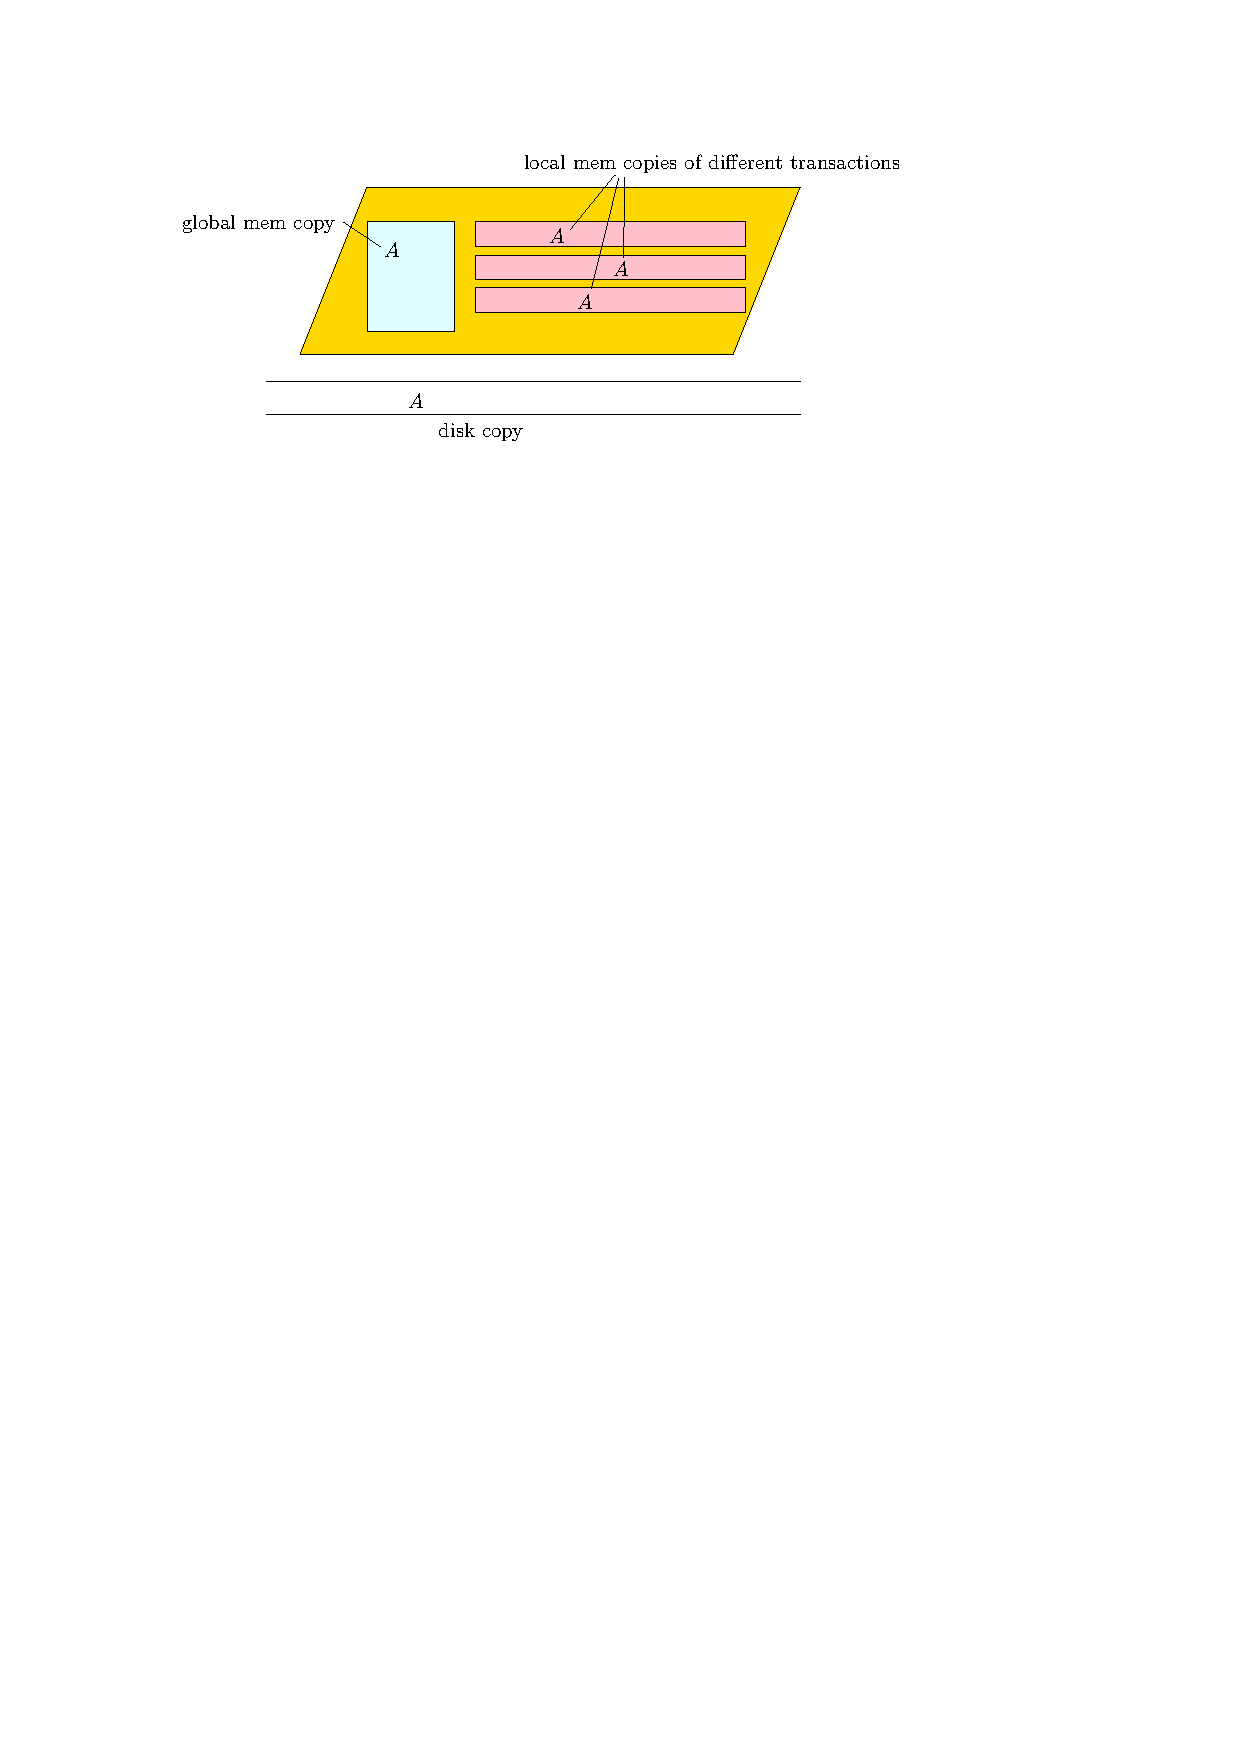
\includegraphics[height=35mm]{./artwork/val-copies}
    \end{center}

}
%-------------------------------------------------------------
\myfrm{
    %\xmybox{Three Copies of the Same Value}

    \cbox{blue}{
    \blue{System-level instructions:}
    \myitems{
        \item $\red{\inp}(A)$: Read the disk copy into the global memory copy.
        \item $\red{\out}(A)$: Write the global memory copy to the disk copy.
    }
    }
    \cbox{blue}{
    \blue{Transaction-level instructions:}
    \myitems{
        \item
        $\red{\rd}(A)$: Read the global memory copy into the local memory copy of a transaction.
    \item
    $\red{\wt}(A)$: Write a transaction's local memory copy to the global memory copy.
    }
    }

    \begin{center}
        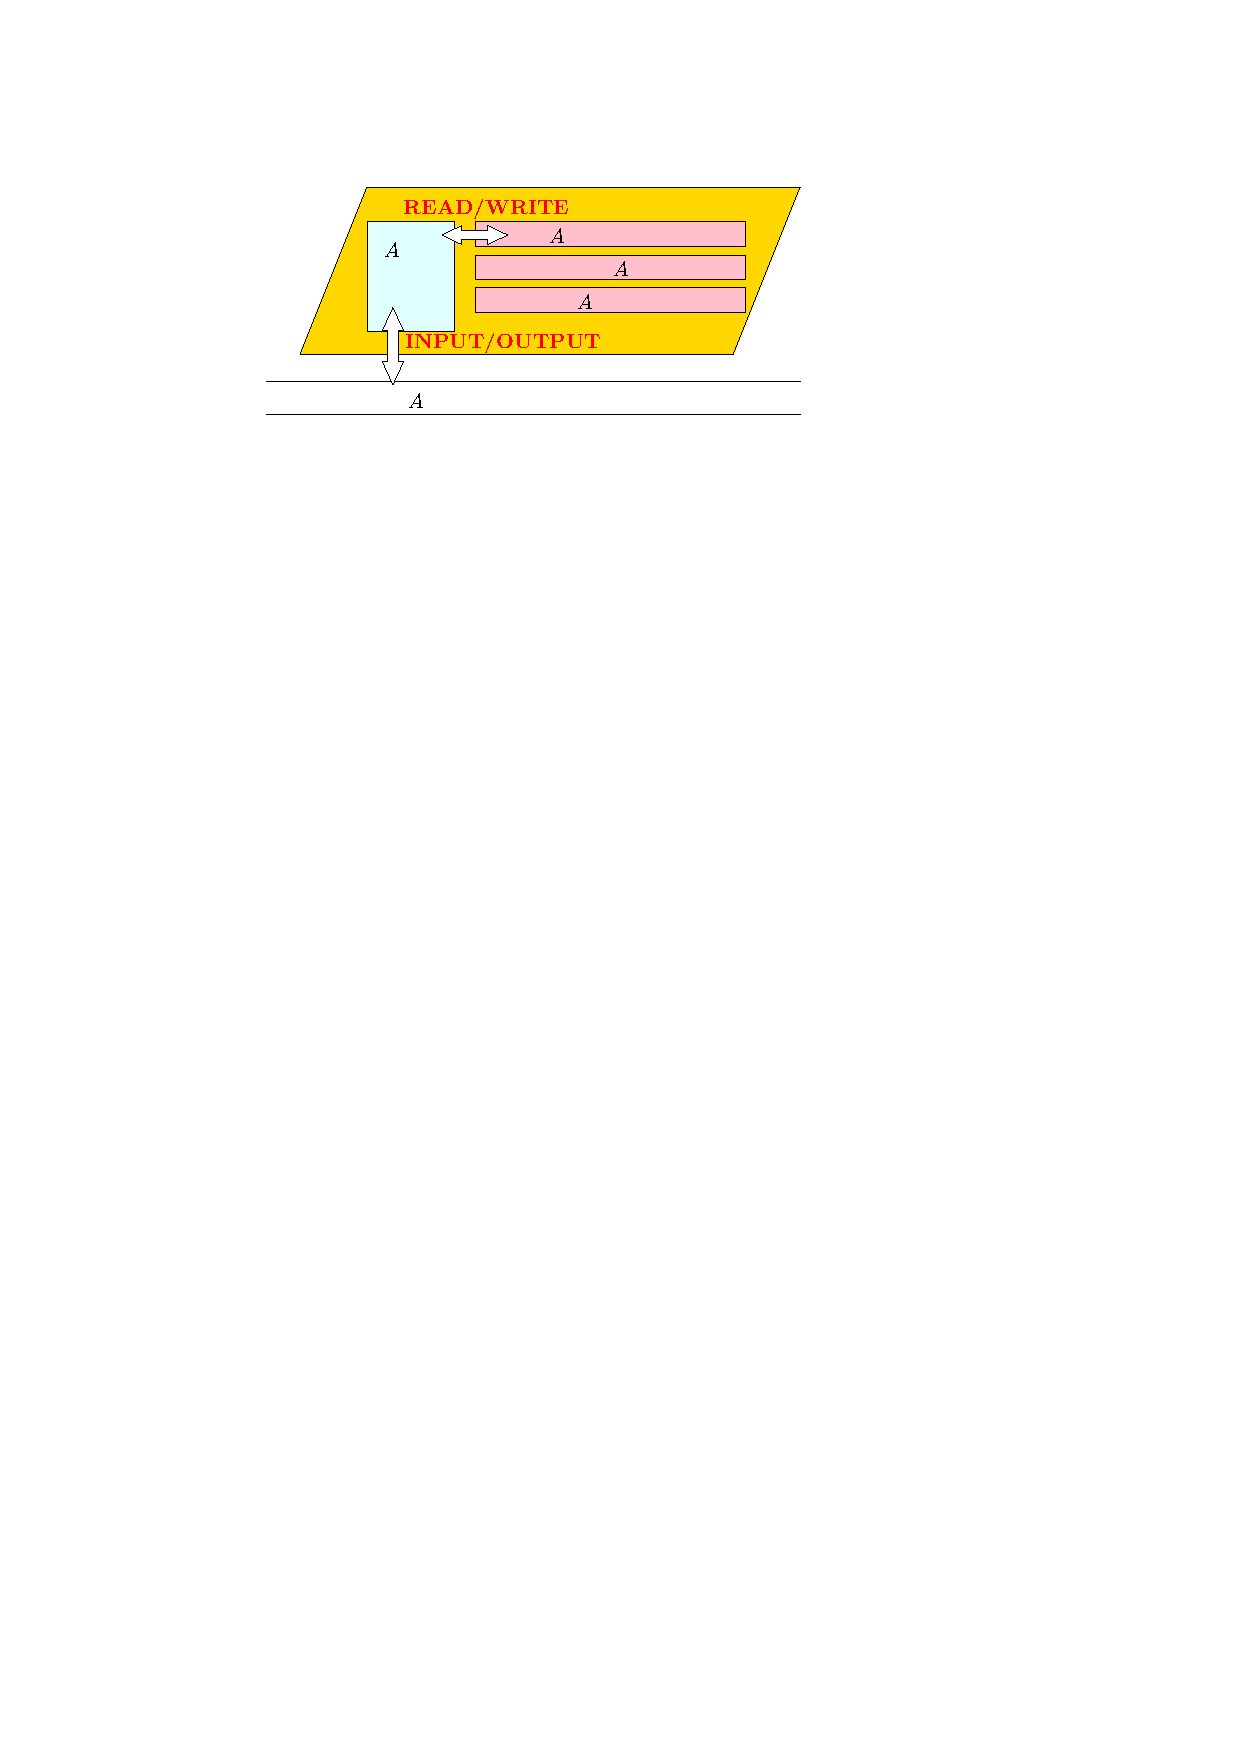
\includegraphics[height=25mm]{./artwork/val-copies2}
    \end{center}

}
%-------------------------------------------------------------
\myfrm{
    \cbox{green}{
        \blue{Example 1 (cont.):} The following shows the schedule \bred{at the system level} and its execution (assuming $\red{A = 10}$ on the disk initially): \vspace{-3mm}

        \begin{center}
        \begin{tabular}{c|c|c|c|c|c}
            step & schedule & \multicolumn{4}{c}{value of $A$} \\
            & & disk & global & $T_1$ local & $T_2$ local \\
            \hline
            0& & 10 & n/a & n/a & n/a \\
            1& $\inp(A)$ & 10 & 10 & n/a & n/a \\
            2& $T_1: \rd(A)$ & 10 & 10 & 10 & n/a \\
            3& $T_1: A = A + 1$ & 10 & 10 & 11 & n/a \\
            4& $T_1: \wt(A)$ & 10 & 11 & 11 & n/a \\
            5& $T_1: \cmt$ & 10 & 11 & n/a & n/a \\
            6& $T_2: \rd(A)$ & 10 & 11 & n/a & 11 \\
            7& $T_2: A = A + 1$ & 10 & 11 & n/a & 12 \\
            8& $T_2: \wt(A)$ & 10 & 12 & n/a & 12 \\
            9& $T_2: \cmt$ & 10 & 12 & n/a & n/a \\
            10& $\out(A)$ & 12 & 12 & n/a & n/a
        \end{tabular}

        \cbox{red}{
            What if a system crashes after step 5? How about after step 8? step 9?
        }
        \end{center}
    }
}
%-------------------------------------------------------------
\myfrm{
    \xmybox{Logging}

    \vgap

    Logging is a standard approach to implement the recovery mechanism in database systems.

    \vgap

    \cbox{blue}{
    A \blue{log file} is a special file on the disk maintained by the system. It contains a sequence of \blue{log records} that capture transactions' behavior.
    }




}
%-------------------------------------------------------------
\myfrm{
    \xmybox{Logging}

    \vgap

    We will introduce three logging methods, which use different sets of log records. However, the following three records are \bred{common to all methods}.

    \myitems{
        \item \red{\dblog{START $T$}}: Records the start of transaction $T$.
        \item \red{\dblog{COMMIT $T$}}: Records that transaction $T$ has committed.
        \item \red{\dblog{ABORT $T$}}: Records that transaction $T$ has aborted.
    }
}
%-------------------------------------------------------------
\myfrm{
    \cbox{yellow}{
        \centering
        Method 1: Undo Logging
    }
}
%-------------------------------------------------------------
\myfrm{
    \xmybox{New Log Records}

    \vgap

    This method allows one more type of log records:

    \myitems{
        \item \red{\dblog{$T$, $A$, $a_{old}$}} \\
        Meaning: transaction $\red{T}$ will change a tuple's attribute $\red{A}$, and the attribute's value is $\red{a_{old}}$ currently.
    }
}
%-------------------------------------------------------------
\myfrm{
    \xmybox{Rules}

    %\vgap

    \cbox{blue}{
        \blue{Rule 1:} When a transaction $\red{T}$ performs $\wt(\red{A})$, create a log record \red{\dblog{$T, A, a_{old}$}}.
    }

    \cbox{blue}{
        \blue{Rule 2:} The disk copy of $A$ can change only \bred{after} the corresponding log record \red{\dblog{$T, A, a_{old}$}} has been written to the disk.
    }

    \cbox{blue}{
        \blue{Rule 3:} The log record \red{\dblog{COMMIT $T$}} can be written to the disk only \bred{after} all the changes of $T$ have been written to the disk.
    }

    \vgap

    Intuitively, the ``correct'' ordering is: \\
    \dblog{$T, A, a_{old}$} $\Rightarrow$ disk copy of $A$ changes $\Rightarrow$ \dblog{COMMIT $T$}
}
%-------------------------------------------------------------
\myfrm{
    \cbox{green}{
        \blue{Example 2:} \vspace{-5mm}

        \begin{center}
        \begin{tabular}{c|c|c|c|c|c}
            step & schedule & disk & global & $T_1$ & log \\
            \hline
            0& & 10 & n/a & n/a & \dblog{START $T_1$} \\
            1& $\inp(A)$ & 10 & 10 & n/a &  \\
            2& $T_1: \rd(A)$ & 10 & 10 & 10 &  \\
            3& $T_1: A = A + 1$ & 10 & 10 & 11 &  \\
            4& $T_1: \wt(A)$ & 10 & 11 & 11 & \dblog{$T_1,A, 10$} \\
            5& $\out(A)$ & 11 & 11 & n/a & \\
            6& $T_1: \cmt$ & 11 & 11 & n/a & \dblog{COMMIT $T_1$}
        \end{tabular}

        \cbox{red}{
            Note: In this schedule, $\out(A)$ appears before $T_1$ commits. This is possible: $\out(A)$ is performed by the system (not by $T_1$). The system may choose to perform the operation any time (as per its buffer management policy).
        }


        \end{center}
    }
}
%-------------------------------------------------------------
\myfrm{
    \xmybox{Recovery from Failure}

    \vgap

    Suppose that the system reboots from a crash.

    %\vgap

    \cbox{blue}{
        The recovery module starts by identifying the transactions that were committed, aborted, and running at the moment of crash.
    }
    \blue{Think:} How?

    \vgap


    \cbox{blue}{
        \blue{Recovery algorithm:} Scan the log \bred{backward}. \\
        For each record \red{\dblog{$T, A, a_{old}$}}, if $T$ did not commit before the crash, set the disk copy of $A$ to $a_{old}$.
    }
}
%-------------------------------------------------------------
\myfrm{
    \cbox{green}{
        \blue{Example 2 (cont.):} Suppose that the system sees the  following log after a crash.

        \begin{center}
        \begin{tabular}{c}
            log \\
            \hline
            \dblog{START $T_1$} \\
            \dblog{$T_1,A, 10$} \\
            \dblog{COMMIT $T_1$}
        \end{tabular}
        \end{center}

        The recovery algorithm does not modify the disk.
    }
}
%-------------------------------------------------------------
\myfrm{
    \cbox{green}{
        \blue{Example 2 (cont.):} Suppose that the system sees the  following log after a crash.

        \begin{center}
        \begin{tabular}{c}
            log \\
            \hline
            \dblog{START $T_1$} \\
            \dblog{$T_1,A, 10$}
        \end{tabular}
        \end{center}

        The recovery algorithm sets the disk copy of $A$ to 10.
    }
}
%-------------------------------------------------------------
\myfrm{
    \cbox{yellow}{
        \centering
        Method 2: Redo Logging
    }
}
%-------------------------------------------------------------
\myfrm{
    \xmybox{New Log Records}

    \vgap

    This method allows one more type of log records:

    \myitems{
        \item \red{\dblog{$T$, $A$, $a_{new}$}} \\
        Meaning: transaction $\red{T}$ will change a tuple's attribute $\red{A}$ to $\red{a_{new}}$.
    }
}
%-------------------------------------------------------------
\myfrm{
    \xmybox{Rules}

    %\vgap

    \cbox{blue}{
        \blue{Rule 1:} When a transaction $\red{T}$ performs $\wt(\red{A})$, create a log record \red{\dblog{$T, A, a_{new}$}}.
    }

    \cbox{blue}{
        \blue{Rule 2:} The log record \red{\dblog{COMMIT $T$}} of $T$ can be written to the disk only \bred{after} the other log records of $T$ have been written to the disk.
    }

    \cbox{blue}{
        \blue{Rule 3:} The changes of $T$ can be written to the disk only \bred{after} \red{\dblog{COMMIT $T$}} has been written to the disk.
    }

    \vgap

    Intuitively, the ``correct'' ordering is: \\
    \dblog{$T, A, a_{new}$} $\Rightarrow$ \dblog{COMMIT $T$} $\Rightarrow$ disk copy of $A$ changes
}
%-------------------------------------------------------------
\myfrm{
    \cbox{green}{
        \blue{Example 3:} \vspace{-5mm}

        \begin{center}
        \begin{tabular}{c|c|c|c|c|c}
            step & schedule & disk & global & $T_1$ & log \\
            \hline
            0& & 10 & n/a & n/a & \dblog{START $T_1$} \\
            1& $\inp(A)$ & 10 & 10 & n/a &  \\
            2& $T_1: \rd(A)$ & 10 & 10 & 10 &  \\
            3& $T_1: A = A + 1$ & 10 & 10 & 11 &  \\
            4& $T_1: \wt(A)$ & 10 & 11 & 11 & \dblog{$T_1,A, 11$} \\
            5& $\out(A)$ & 11 & 11 & n/a & \\
            6& $T_1: \cmt$ & 11 & 11 & n/a & \dblog{COMMIT $T_1$}
        \end{tabular}


        \end{center}
    }
}
%-------------------------------------------------------------
\myfrm{
    \xmybox{Recovery from Failure}

    \vgap

    Suppose that the system reboots from a crash.

    %\vgap

    \cbox{blue}{
        The recovery module starts by identifying the transactions that were committed, aborted, and running at the moment of crash.
    }
    %\blue{Think:} How?

    \vgap


    \cbox{blue}{
        \blue{Recovery algorithm:} Scan the log \bred{forward}. \\
        For each record \red{\dblog{$T, A, a_{new}$}}, if $T$ had committed before the crash, set the disk copy of $A$ to $a_{new}$.
    }
}
%-------------------------------------------------------------
\myfrm{
    \cbox{green}{
        \blue{Example 2 (cont.):} Suppose that the system sees the  following log after a crash.

        \begin{center}
        \begin{tabular}{c}
            log \\
            \hline
            \dblog{START $T_1$} \\
            \dblog{$T_1,A, 11$} \\
            \dblog{COMMIT $T_1$}
        \end{tabular}
        \end{center}

        The recovery algorithm sets the disk copy of $A$ to 11.
    }
}
%-------------------------------------------------------------
\myfrm{
    \cbox{green}{
        \blue{Example 3 (cont.):} Suppose that the system sees the  following log after a crash.

        \begin{center}
        \begin{tabular}{c}
            log \\
            \hline
            \dblog{START $T_1$} \\
            \dblog{$T_1,A, 10$}
        \end{tabular}
        \end{center}

        The recovery algorithm does not modify the disk.
    }
}
%-------------------------------------------------------------
\myfrm{
    \cbox{yellow}{
        \centering
        Method 3: Undo/Redo Logging
    }
}
%-------------------------------------------------------------
\myfrm{
    \xmybox{New Log Records}

    \vgap

    This method allows one more type of log records:

    \myitems{
        \item \red{\dblog{$T$, $A$, $a_{old}$, $a_{new}$}} \\
        Meaning: transaction $\red{T}$ will change a tuple's attribute $\red{A}$ to $\red{a_{new}}$, and the attribute's value is $\red{a_{old}}$ currently.
    }
}
%-------------------------------------------------------------
\myfrm{
    \xmybox{Rules}

    %\vgap

    \cbox{blue}{
        \blue{Rule 1:} When a transaction $\red{T}$ performs $\wt(\red{A})$, create a log record \red{\dblog{$T, A, a_{old}, a_{new}$}}.
    }

    \cbox{blue}{
        \blue{Rule 2:} The disk copy of $A$ can change to $\red{a_{new}}$ only \bred{after} the corresponding log record \red{\dblog{$T, A, a_{old}, a_{new}$}} has be written to the disk.
    }

    \cbox{blue}{
        \blue{Rule 3:} The log record \red{\dblog{COMMIT $T$}} of $T$ can be written to the disk only \bred{after} the other log records of $T$ have been written to the disk.
    }

    %\vgap

    Intuitively, the ``correct'' ordering is: \\
    \dblog{$T, A, a_{new}$} $\Rightarrow$ \dblog{COMMIT $T$} \\
    \dblog{$T, A, a_{new}$} $\Rightarrow$ disk copy of $A$ changes \\
    The ordering between \dblog{COMMIT $T$} and disk-copy changes does not matter.
}
%-------------------------------------------------------------
\myfrm{
    \cbox{green}{
        \blue{Example 4:} \vspace{-5mm}

        \begin{center}
        \begin{tabular}{c|c|c|c|c|c}
            step & schedule & disk & global & $T_1$ & log \\
            \hline
            0& & 10 & n/a & n/a & \dblog{START $T_1$} \\
            1& $\inp(A)$ & 10 & 10 & n/a &  \\
            2& $T_1: \rd(A)$ & 10 & 10 & 10 &  \\
            3& $T_1: A = A + 1$ & 10 & 10 & 11 &  \\
            4& $T_1: \wt(A)$ & 10 & 11 & 11 & \dblog{$T_1,A, 10, 11$} \\
            5& $\out(A)$ & 11 & 11 & n/a & \\
            6& $T_1: \cmt$ & 11 & 11 & n/a & \dblog{COMMIT $T_1$}
        \end{tabular}


        \end{center}
    }
}
%-------------------------------------------------------------
\myfrm{
    \xmybox{Recovery from Failure}

    \vgap

    Suppose that the system reboots from a crash.

    %\vgap

    \cbox{blue}{
        The recovery module starts by identifying the transactions that were committed, aborted, and running at the moment of crash.
    }
    %\blue{Think:} How?

    \vgap


    \cbox{blue}{
        \blue{Recovery algorithm:} \\
        Scan the log \bred{backward}.
        For each record \red{\dblog{$T, A, a_{old}, a_{new}$}}, if $T$ did \bred{not} commit before the crash, set the disk copy of $A$ to $a_{old}$.

        \vgap

        Scan the log \bred{forward}.
        For each record \red{\dblog{$T, A, a_{old}, a_{new}$}}, if $T$ had \bred{committed} before the crash, set the disk copy of $A$ to $a_{new}$.
    }
}
%-------------------------------------------------------------
\myfrm{
    \cbox{green}{
        \blue{Example 4 (cont.):} Suppose that the system sees the  following log after a crash.

        \begin{center}
        \begin{tabular}{c}
            log \\
            \hline
            \dblog{START $T_1$} \\
            \dblog{$T_1, A, 10, 11$} \\
            \dblog{COMMIT $T_1$}
        \end{tabular}
        \end{center}

        The recovery algorithm sets the disk copy of $A$ to 11.
    }
}
%-------------------------------------------------------------
\myfrm{
    \cbox{green}{
        \blue{Example 3 (cont.):} Suppose that the system sees the  following log after a crash.

        \begin{center}
        \begin{tabular}{c}
            log \\
            \hline
            \dblog{START $T_1$} \\
            \dblog{$T_1,A, 10, 11$}
        \end{tabular}
        \end{center}

        The recovery algorithm sets the disk copy of $A$ to 10.
    }
}
%-------------------------------------------------------------
\end{document} 



